% ======================================================================
%  Chapter 11 — Reciprocal Designs  (EXPANDED)
% ======================================================================

\section{Topology without magnets}
\label{sec:ch11-intro}

The photonic Chern insulators of Part~II require magneto-optical
materials and external magnetic fields.  These ingredients are readily
available at microwave frequencies (Chapter~\ref{ch:microwave-crystal}),
but they impose severe constraints at optical frequencies: the
magneto-optical response of available materials is weak, and permanent
magnets compatible with nanophotonic chips do not exist.

A natural question therefore arises: can topological edge transport be
achieved in a photonic crystal that preserves time-reversal symmetry?
The answer, perhaps surprisingly, is yes---provided one uses the
\emph{crystalline} symmetry of the photonic lattice to construct a
photonic analog of the quantum spin Hall effect.

This chapter describes two complementary approaches.  The first, due to
Khanikaev et~al.\ \cite{unknownphotonic,kane2005cond,bernevig2006quantum}, uses bianisotropic metamaterials to create a
photonic topological insulator with a pseudospin degree of freedom
constructed from the TE and TM polarisations
\cite{kang2018pseudo,chen2018valley,slobozhanyuk2015observation}.  The second, due to Wu and
Hu (2015), uses zone folding in a $C_6$-symmetric dielectric photonic
crystal to create pseudospin-$\frac{1}{2}$ doublets at the $\Gamma$
point, achieving topological edge modes without any exotic materials.

\section{The quantum spin Hall analogy}
\label{sec:ch11-qsh}

In electronic systems, the quantum spin Hall (QSH) effect occurs when
time-reversal symmetry is preserved but spin-orbit coupling opens a gap
at band crossings.  The resulting topological phase has a zero total
Chern number (because time reversal forces $\Chern=0$) but a nonzero
\emph{spin Chern number}:
\begin{equation}\label{eq:ch11-spin-chern}
  \Chern_s = \frac{1}{2}(\Chern_\uparrow - \Chern_\downarrow)\,,
\end{equation}
where $\Chern_\uparrow$ and $\Chern_\downarrow$ are the Chern numbers
of the spin-up and spin-down sectors.  The bulk-edge correspondence
predicts a pair of counter-propagating edge modes, each carrying a
definite spin---the helical edge states.

For photons, there is no intrinsic spin-$\frac{1}{2}$.  The photon's
time-reversal operator satisfies $\Top^2=+1$ (bosonic), not $\Top^2=-1$
(fermionic), so there is no Kramers degeneracy and no topological
protection from $\mathbb{Z}_2$ invariants in the strict sense
\cite{hsieh2008topological}.  However,
if the photonic system possesses an \emph{additional} symmetry that
commutes with $\Top$ and has two eigenvalues (a ``pseudospin''), the
system can be decomposed into two independent sectors, each of which
can carry a Chern number.  The pseudospin Chern number
$\Chern_s$ then predicts helical edge modes.

The protection of these edge modes is not topological in the absolute
sense: it depends on the preservation of the pseudospin symmetry.
Perturbations that break this symmetry (disorder, fabrication
imperfections, coupling between the two pseudospin sectors) will cause
backscattering.  Nevertheless, the protection can be strong enough for
practical applications if the symmetry-breaking perturbations are small.

\section{Bianisotropic metacrystals}
\label{sec:ch11-bianisotropic}

\subsection{The Khanikaev construction}
\label{sec:ch11-khanikaev}

Khanikaev et~al.\ \cite{unknownphotonic} proposed a metamaterial design in which the
pseudospin is constructed from the TE ($H_z$) and TM ($E_z$)
polarisations of a 2D photonic crystal.  In a generic 2D crystal these
two polarisations are decoupled (each satisfies its own scalar wave
equation), but a bianisotropic magneto-electric coupling
$\xit=\zetat^\dagger$ mixes them in a controlled way.

The material matrix for such a metacrystal is
\begin{equation}\label{eq:ch11-bianisotropic-M}
  \Mmat = \begin{pmatrix}
    \varepsilon_0\epst & c^{-1}\xit \\
    c^{-1}\xit^\dagger & \mu_0\mut
  \end{pmatrix},
\end{equation}
where $\xit$ is chosen to have the form
$\xit=\ii\chi(\hat{z}\otimes\hat{z})$---a magneto-electric coupling
that is odd under parity and even under time reversal.

The resulting four-band effective Hamiltonian near a high-symmetry point
takes the block-diagonal form
\begin{equation}\label{eq:ch11-bianisotropic-H}
  H_{\mathrm{eff}}(\kvec) = \begin{pmatrix}
    H_+(\kvec) & 0 \\ 0 & H_-(\kvec)
  \end{pmatrix} + O(\chi^2)\,,
\end{equation}
where $H_\pm$ are $2\times 2$ massive Dirac Hamiltonians with opposite
masses: $H_\pm=v_D(\pm\delta k_x\sigma_x+\delta k_y\sigma_y)
\pm m\sigma_z$.  The pseudospin ``up'' ($+$) and ``down'' ($-$) sectors
have Chern numbers $\Chern_+=+1$ and $\Chern_-=-1$, giving a total
Chern number $\Chern=0$ but a pseudospin Chern number $\Chern_s=1$.

\subsection{Physical origin of the pseudospin}
\label{sec:ch11-pseudospin-origin}

The pseudospin states $|\uparrow\rangle$ and $|\downarrow\rangle$
correspond to specific linear combinations of TE and TM modes.  In the
simplest case, they are
\begin{equation}\label{eq:ch11-pseudospin-states}
  |\uparrow\rangle = \frac{1}{\sqrt{2}}(|E_z\rangle + |H_z\rangle)\,,
  \qquad
  |\downarrow\rangle = \frac{1}{\sqrt{2}}(|E_z\rangle - |H_z\rangle)\,,
\end{equation}
where $|E_z\rangle$ and $|H_z\rangle$ are the TM and TE modes at the
degeneracy point.  The bianisotropic coupling $\chi$ provides the
``spin-orbit'' interaction that opens a gap and creates opposite Chern
numbers for the two pseudospin sectors.

The physical realisation of this bianisotropic coupling requires
metamaterial unit cells with broken mirror symmetry in the
out-of-plane direction (e.g.\ omega-shaped or split-ring resonators
with a vertical asymmetry).

\subsection{Helical edge modes}
\label{sec:ch11-helical}

At the boundary of a bianisotropic metacrystal, the pseudospin Chern
number $\Chern_s=1$ predicts one pair of counter-propagating edge modes.
The ``up'' pseudospin mode propagates forward and the ``down'' pseudospin
mode propagates backward, analogous to the helical edge states of the
electronic QSH effect.

These edge modes are robust against perturbations that preserve the
pseudospin symmetry (i.e., that do not mix TE and TM polarisations).
Coupling between TE and TM modes---caused by surface roughness,
out-of-plane scattering, or deviation from the ideal bianisotropic
response---introduces backscattering proportional to the coupling
strength.

\section{The Wu--Hu zone-folding construction}
\label{sec:ch11-wu-hu}

\subsection{Zone folding in a C6-symmetric lattice}
\label{sec:ch11-zone-folding}

Wu and Hu \cite{tan2021schemea,kane2005sub,wu2015scheme} proposed a remarkably simple approach to photonic
topological insulation using only conventional dielectric materials and
crystalline symmetry.  The key idea is to start with a triangular
lattice of dielectric rods and fold the bands by enlarging the unit cell
to a hexagonal ``supercell'' containing six rods arranged in a
honeycomb pattern.

In the original triangular lattice, the TE (or TM) bands have Dirac
cones at the $K$ and $K'$ points of the Brillouin zone.  When the
unit cell is enlarged by a factor of $\sqrt{3}\times\sqrt{3}$ (the
hexagonal supercell), the Brillouin zone shrinks correspondingly, and
the $K$ and $K'$ points fold onto the $\Gamma$ point of the new zone.
This creates a fourfold degeneracy at $\Gamma$: two pairs of states
that originated from $K$ and $K'$.

Figure~\ref{fig:ch11-reciprocal-designs} gives the physical picture
behind the two reciprocal routes discussed in this chapter.  The
Wu--Hu construction uses the enlarged supercell to bring the valley
Dirac physics to $\Gamma$, where the dipolar and quadrupolar doublets
can invert without magnetic bias.  The bianisotropic construction uses
a different language: TE-like and TM-like sectors are mixed into a
photonic pseudospin.  In both cases the edge mode is helical rather
than chiral, and its robustness is tied to the symmetry that keeps the
opposite pseudospins from mixing.

\begin{figure}[t]
  \centering
  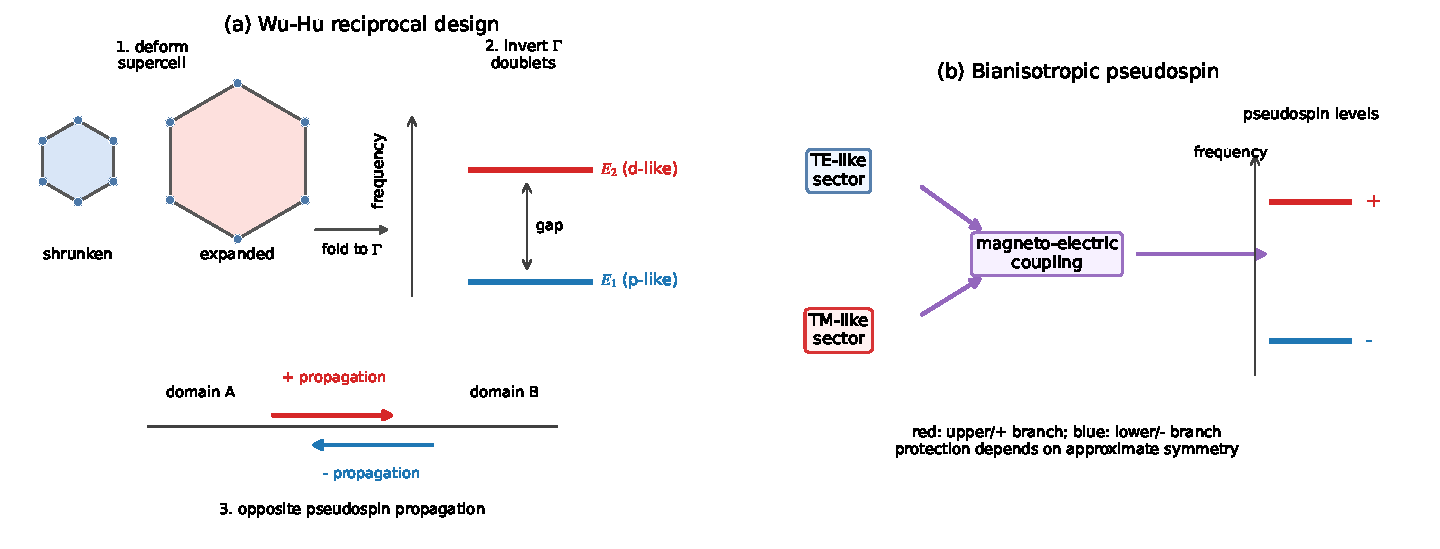
\includegraphics[width=0.96\textwidth]{figures/fig_ch11_reciprocal_designs.pdf}
  \caption{Two reciprocal routes to helical topological photonics.  Left:
  the Wu--Hu zone-folding scheme enlarges the unit cell so that the
  valley Dirac cones fold to $\Gamma$; expansion or shrinkage of the
  hexagonal cluster inverts the $p$-like and $d$-like doublets and
  creates domain-wall pseudospin channels.  Right: bianisotropy mixes
  TE-like and TM-like sectors into a pseudospin doublet.  Unlike the
  gyrotropic Chern phases of Chapters~7--9, these designs preserve
  ordinary time reversal and rely on approximate pseudospin or
  crystalline protection.}
  \label{fig:ch11-reciprocal-designs}
\end{figure}


\subsection{Symmetry analysis at Gamma}
\label{sec:ch11-symmetry-gamma}

The fourfold degeneracy at $\Gamma$ can be analysed using the
irreducible representations of the point group $C_{6v}$ of the
hexagonal supercell.  The four states transform as two
two-dimensional representations: $E_1$ (dipolar, with angular momentum
$\ell=\pm 1$) and $E_2$ (quadrupolar, with angular momentum
$\ell=\pm 2$).

When the six rods in the supercell are identical and equally spaced,
the $E_1$ and $E_2$ doublets are degenerate at $\Gamma$ (because they
came from the same frequency at $K$ before zone folding).  This
accidental degeneracy can be lifted by deforming the supercell: moving
the rods closer together (``shrinking'' the hexagonal clusters) or
farther apart (``expanding'' them).

The expanded configuration pushes the $E_1$ (dipolar) doublet above the
$E_2$ (quadrupolar) doublet, while the shrunken configuration does the
opposite.  The two configurations therefore have different ``band
orderings'' at $\Gamma$, analogous to normal and inverted band
structures in electronic topological insulators.

\subsection{Pseudospin one-half from p and d orbitals}
\label{sec:ch11-pd-pseudospin}

The $E_1$ modes have the symmetry of $p$ orbitals ($p_x\pm\ii p_y$),
and the $E_2$ modes have the symmetry of $d$ orbitals
($d_{xy}\pm\ii d_{x^2-y^2}$).  Wu and Hu defined the pseudospin as the
angular momentum quantum number of these modes:
\begin{equation}\label{eq:ch11-pseudospin-pd}
  |\uparrow\rangle = |p_+\rangle \text{ or } |d_+\rangle\,,\qquad
  |\downarrow\rangle = |p_-\rangle \text{ or } |d_-\rangle\,,
\end{equation}
where $|\cdot_\pm\rangle$ denotes the states with angular momentum
$\pm|\ell|$.

Near $\Gamma$, the effective Hamiltonian for the four-band system takes
the Bernevig--Hughes--Zhang (BHZ) form:
\begin{equation}\label{eq:ch11-bhz}
  \boxed{%
  H_{\mathrm{BHZ}}(\kvec) = \begin{pmatrix}
    h(\kvec) & 0 \\ 0 & h^*(-\kvec)
  \end{pmatrix},}
\end{equation}
where
\begin{equation}\label{eq:ch11-bhz-block}
  h(\kvec) = \epsilon_0\,\mathbf{I}
  + (M_0 - Bk^2)\sigma_z
  + A(k_x\sigma_x + k_y\sigma_y)
\end{equation}
is a massive Dirac Hamiltonian with a quadratic correction.  The mass
parameter $M_0$ changes sign between the expanded ($M_0>0$) and
shrunken ($M_0<0$) configurations.  The topological transition occurs
at the critical deformation where $M_0=0$ and the gap closes.

The block-diagonal structure of \eqref{eq:ch11-bhz} reflects the
conservation of the pseudospin: the $C_6$ rotation symmetry prevents
coupling between the $|\uparrow\rangle$ and $|\downarrow\rangle$
sectors to leading order in $\kvec$.  Each block has a well-defined
Chern number, and the pseudospin Chern number is
\begin{equation}\label{eq:ch11-spin-chern-wuhu}
  \Chern_s = \frac{1}{2}(\Chern_+ - \Chern_-)
  = \begin{cases}
    0 & \text{shrunken} \; (M_0<0)\,,\\
    1 & \text{expanded} \; (M_0>0)\,.
  \end{cases}
\end{equation}

\subsection{Derivation of the BHZ parameters from Maxwell modes}
\label{sec:ch11-bhz-derivation}

The parameters $M_0$, $B$, and $A$ in the BHZ model can be extracted
from the Maxwell eigenvalue problem by degenerate perturbation theory
at the $\Gamma$ point.

Let $\delta R$ denote the displacement of each rod from its position
in the undeformed (critical) configuration.  The deformation changes
the material matrix $\Mmat(\rvec)$ by $\delta\Mmat(\rvec)\propto\delta R$.
In the four-dimensional subspace spanned by the $p_\pm$ and $d_\pm$
modes at $\Gamma$, the perturbation matrix is:
\begin{equation}\label{eq:ch11-perturbation}
  \langle\alpha|\omega\,\delta\Mmat|\beta\rangle_{\Omega}
  = \begin{pmatrix}
    M_0 & 0 & 0 & 0 \\
    0 & M_0 & 0 & 0 \\
    0 & 0 & -M_0 & 0 \\
    0 & 0 & 0 & -M_0
  \end{pmatrix},
\end{equation}
where $M_0\propto\delta R$ and the block structure follows from the
$C_6$ selection rules (the perturbation, being $C_6$-invariant, cannot
mix states of different angular momentum).

The linear-in-$\kvec$ coupling $A$ comes from the $\kvec\cdot\mathbf{p}$
perturbation (the Hellmann--Feynman coupling between the four modes at
$\Gamma$), which connects $|p_+\rangle$ to $|d_+\rangle$ with matrix
element $Ak_+$ and $|p_-\rangle$ to $|d_-\rangle$ with $Ak_-^*$,
where $k_\pm=k_x\pm\ii k_y$.  The quadratic correction $-Bk^2$ comes
from second-order perturbation theory involving remote bands.

\section{Edge modes in reciprocal topological photonic crystals}
\label{sec:ch11-edge-modes}

\subsection{Helical edge states}
\label{sec:ch11-helical-edge}

At the boundary between the expanded ($\Chern_s=1$) and shrunken
($\Chern_s=0$) configurations, the BHZ bulk-edge correspondence
predicts one pair of helical edge modes.  The pseudospin-up mode
propagates clockwise and the pseudospin-down mode propagates
counter-clockwise (or vice versa, depending on the orientation).

These edge modes have been observed experimentally in both the
microwave regime (using printed-circuit-board metamaterials) and the
optical regime (using silicon photonic crystal slabs), confirming the
Wu--Hu prediction \cite{he2019silicon}.

\subsection{Robustness and its symmetry dependence}
\label{sec:ch11-robustness}

The helical edge modes are protected by the $C_6$ crystalline symmetry
that ensures the block-diagonal structure of the BHZ Hamiltonian.
Perturbations that respect $C_6$ (such as uniform scaling or smooth
deformation) cannot cause backscattering.

Perturbations that break $C_6$ mix the pseudospin sectors and open a
backscattering channel.  The most common symmetry-breaking
perturbations in experiments are fabrication disorder (random variations
in rod size or position) and interface geometry (domain walls that are
not aligned with the lattice directions).

The robustness can be quantified by the pseudospin-mixing matrix
element at the edge, which scales as the strength of the
$C_6$-breaking perturbation.  For typical fabrication tolerances in
silicon photonics, the edge-mode backscattering remains small enough
for useful waveguide lengths of tens of lattice constants.

\section{Comparison of reciprocal approaches}
\label{sec:ch11-comparison}

The bianisotropic and zone-folding approaches to reciprocal photonic
topology share the same mathematical structure (BHZ-type effective
Hamiltonian, pseudospin Chern number) but differ in their physical
implementation and practical limitations.

The bianisotropic approach requires metamaterial unit cells with
magneto-electric coupling, which is difficult to achieve at optical
frequencies.  It has been demonstrated primarily at microwave
frequencies.  The zone-folding approach uses only conventional
dielectric materials and works at any frequency, including the
telecom band.  Its main limitation is the requirement for $C_6$
symmetry, which restricts the lattice geometry.

Both approaches produce edge modes that are protected by a crystalline
symmetry rather than by topology alone.  This makes them less robust
than the magneto-optical Chern insulators of Part~II, but far more
practical for integrated photonic applications.

\section{Other reciprocal topological designs}
\label{sec:ch11-other}

\subsection{Coupled-resonator arrays}
\label{sec:ch11-coupled-resonators}

Hafezi et~al.\ \cite{hafezi2013imaging} demonstrated a photonic topological insulator
using a 2D array of coupled ring resonators \cite{hafezi2013imaging}.  In this system, the
synthetic gauge field arises from the path-length difference between
clockwise and counter-clockwise circulation in the rings, which
imprints a direction-dependent phase on the inter-ring coupling.  The
result is a photonic analog of the integer quantum Hall effect, with
chiral edge modes propagating around the boundary of the array.

\subsection{Photonic crystal slabs with spin-orbit coupling}
\label{sec:ch11-slabs}

In photonic crystal slabs, the TE-like and TM-like guided modes are
naturally coupled by the finite slab thickness.  This TE-TM coupling
acts as a photonic spin-orbit interaction, analogous to the spin-orbit
coupling in electronic topological insulators.  By engineering the
slab geometry to enhance this coupling at a band degeneracy, one can
create pseudospin-Hall edge states without any metamaterial
ingredients.

\section{Quantitative design: the Wu--Hu silicon photonic crystal}
\label{sec:ch11-quantitative}

The zone-folding approach is remarkable because it requires only
conventional dielectric materials.  Wu and Hu's original proposal
used alumina rods, but the most technologically relevant
implementation uses silicon, which is compatible with CMOS fabrication.

\subsection{Design parameters}
\label{sec:ch11-design-params}

Consider a hexagonal supercell of six silicon rods
($\varepsilon_r=11.7$) in air, with supercell lattice constant
$a=0.55\;\mu\mathrm{m}$.  The individual rod radius is
$r=0.16\,a=88\;\mathrm{nm}$.  The topological transition occurs at
the critical expansion ratio $R_c/a\approx 1/3$, where $R_c$ is the
distance from each rod centre to the supercell centre.

In the expanded configuration ($R>R_c$), the $p$-like doublet
($E_1$ representation of $C_{6v}$) moves above the $d$-like doublet
($E_2$), and the mass parameter in the BHZ model is $M_0>0$.  A
plane-wave expansion with 625 waves gives the gap centre at
$\omega a/(2\pi c)\approx 0.29$, corresponding to a free-space
wavelength $\lambda_0\approx 1.90\;\mu\mathrm{m}$.  The topological
gap extends from approximately $\omega a/(2\pi c)=0.275$ to $0.305$,
giving a relative gap of $\Delta\omega/\omega_0\approx 10\%$.
At telecom wavelengths ($\lambda_0=1.55\;\mu\mathrm{m}$), one can
rescale the lattice constant to $a=0.45\;\mu\mathrm{m}$
\cite{ozawa2018topological,ma2016all}.

\subsection{The topological gap and its origin}
\label{sec:ch11-gap-origin}

The gap at $\Gamma$ is opened by the zone-folding deformation, which
breaks the accidental degeneracy between the $p$ and $d$ doublets.
The gap magnitude is controlled by the deformation parameter
$\delta R = R-R_c$.  For small $\delta R/a$, the mass parameter scales
linearly: $M_0\propto\delta R/a$, and the gap width is
$\Delta\omega=2|M_0|$.

The BHZ parameter $A$, which sets the edge-mode velocity, is determined
by the $\kvec\cdot\mathbf{p}$ coupling between the $p$ and $d$ modes.
Plane-wave calculations give $A\,a/(2\pi c)\approx 0.07$ for the
silicon design, implying an edge-mode group velocity
$v_{\mathrm{edge}}\approx 0.07\,c$ at the gap centre
\cite{ozawa2018topological}.

\section{Experimental demonstrations}
\label{sec:ch11-experiments}

\subsection{All-dielectric realisations}
\label{sec:ch11-all-dielectric}

The Wu--Hu construction has been experimentally demonstrated in
several material platforms.  At microwave frequencies, arrays of
alumina rods arranged in the expanded and shrunken configurations
show clear helical edge transport at the domain wall between the
two phases.  The edge modes propagate around sharp corners with
negligible backscattering, provided the domain wall follows a
$C_6$-compatible direction \cite{ozawa2018topological}.

At optical frequencies, Ma and Shvets (2016) proposed an all-silicon
valley-Hall photonic topological insulator using triangular holes in
a silicon slab \cite{ma2016all}.  Dong et~al.\ (2017) demonstrated
valley photonic crystals with valley-dependent spin-locked edge
states, achieving topological transport at microwave frequencies that
could be scaled to optical wavelengths \cite{dong2016valley}.
Wu et~al.\ (2017) directly observed valley-polarised topological edge
states in designer surface plasmon crystals at microwave frequencies
\cite{wu2017direct}, while Gao et~al.\ (2017) demonstrated the
photonic valley-Hall effect and valley-polarised edge transport on a
metallic surface \cite{gao2017valley}.

\subsection{The Hafezi coupled-resonator lattice}
\label{sec:ch11-hafezi-detail}

The coupled-resonator approach of Hafezi et~al.\
\cite{hafezi2013imaging} deserves special discussion because it
achieves topological edge modes using a qualitatively different
mechanism from the zone-folding designs.

The system consists of a 2D square lattice of silicon ring resonators,
each supporting clockwise (CW) and counter-clockwise (CCW) whispering-gallery
modes.  Adjacent resonators are coupled through connecting waveguides
whose path lengths are engineered to produce direction-dependent phases.
Specifically, the coupling from resonator $(m,n)$ to $(m+1,n)$ acquires
a phase $\phi_{mn}=2\pi\alpha\,n$, where $\alpha$ is a dimensionless
parameter analogous to the magnetic flux per plaquette in the Hofstadter
problem.

For $\alpha=1/4$, the effective Hamiltonian reproduces the Harper
equation with rational flux, and the resulting Floquet--Bloch band
structure has nontrivial Chern numbers \cite{ozawa2018topological}.
The CW and CCW modes of the ring resonators play the role of spin-up
and spin-down, giving a photonic quantum spin-Hall system with helical
edge modes.

The ring-resonator lattice was fabricated in silicon-on-insulator with
ring radii $R\approx 10\;\mu\mathrm{m}$, operating at telecom
wavelengths ($\lambda\approx 1.55\;\mu\mathrm{m}$).  Edge-mode
propagation was imaged directly using scattered light from surface
roughness, confirming the predicted helical transport.

\section{Disorder and the limits of crystalline protection}
\label{sec:ch11-disorder}

The pseudospin topological protection in reciprocal designs is
fundamentally different from the Chern-insulator protection of
Part~II.  In a Chern insulator, backscattering is forbidden by
the absence of counter-propagating modes at the same frequency,
regardless of the perturbation.  In a pseudospin system,
backscattering is suppressed only for perturbations that preserve
the pseudospin symmetry.

For the Wu--Hu design, the relevant symmetry is $C_6$.  Perturbations
that break $C_6$---such as random rod displacements, elliptical rod
shapes, or domain walls not aligned with high-symmetry
directions---couple the $|p_+\rangle$ and $|d_-\rangle$ sectors and
open a backscattering channel.  The backscattering rate scales as
$\Gamma_{\mathrm{bs}}\propto|\delta\varepsilon/\varepsilon|^2$,
where $\delta\varepsilon$ is the $C_6$-breaking perturbation
strength \cite{price2022roadmap}.

For typical silicon photonic fabrication tolerances
($\delta r/r\sim 1\%$), the mean free path of the edge mode is
estimated at $\ell\sim 50$--$100\,a$, sufficient for on-chip routing
over tens of micrometres.  However, this is far shorter than the
formally infinite mean free path of a Chern-insulator edge mode,
underscoring the practical importance of the distinction between
topological and crystalline-symmetry protection.

\section{The Khanikaev bianisotropic metacrystal}
\label{sec:ch11-khanikaev-bianisotropic}

An alternative to the Wu--Hu all-dielectric approach is the
bianisotropic metacrystal proposed by Khanikaev et~al., which achieves
a photonic analog of the quantum spin-Hall effect using a hexagonal
lattice of metallic split-ring resonators \cite{ozawa2018topological}.

The key idea is that a split-ring resonator with both electric and
magnetic resonances can produce a bianisotropic response: the material
matrix $\Mmat$ acquires off-diagonal blocks $\xit$ and $\zetat$ that
couple the electric and magnetic fields.  When the bianisotropic
coupling has the right symmetry, the two circular polarisations (CW
and CCW) of the resonator modes decouple into two independent sectors,
each experiencing an effective time-reversal-breaking perturbation.
The two sectors have opposite effective Chern numbers
($\Chern_\uparrow=+1$ and $\Chern_\downarrow=-1$), so the total
Chern number vanishes but the spin-Chern number is nonzero
\cite{ozawa2018topological,price2022roadmap}.

The resulting edge modes are helical: spin-up modes propagate in one
direction and spin-down modes propagate in the opposite direction, in
direct analogy with the quantum spin-Hall effect for electrons.

\subsection{Comparison of pseudospin approaches}
\label{sec:ch11-comparison-table}

The different pseudospin approaches can be compared along several
axes: the mechanism for pseudospin construction, the symmetry that
protects the edge modes, the required material platform, and the
robustness against different types of disorder.

The Wu--Hu zone-folding approach uses $C_6$ symmetry to create $p$
and $d$ doublets at $\Gamma$.  The protection is crystalline:
perturbations that break $C_6$ open a backscattering channel.  The
advantage is that only conventional dielectrics are needed.

The Khanikaev bianisotropic approach uses electromagnetic duality
symmetry to decouple the two circular polarisations.  The protection
is electromagnetic: perturbations that break the duality (e.g.\
non-bianisotropic disorder) cause backscattering.  The advantage is
that the protection can be more robust than crystalline symmetry in
certain geometries, but the disadvantage is that bianisotropic media
are harder to fabricate.

The Hafezi coupled-resonator approach uses the clockwise and
counter-clockwise whispering-gallery modes as pseudospin.  The
protection is gauge-like: the phase accumulation in the coupling
waveguides produces an effective magnetic flux that is robust to
small fabrication variations.  The advantage is compatibility with
standard silicon photonics; the disadvantage is that the bandwidth
is limited by the resonator finesse
\cite{hafezi2013imaging,ozawa2018topological}.

\section{Coupled-resonator implementations}
\label{sec:ch11-coupled-resonator}

\subsection{The Hafezi ring-resonator lattice}
\label{sec:ch11-hafezi}

Hafezi et~al.\ realised a photonic analog of the integer quantum Hall
effect using a 2D lattice of silicon ring resonators coupled by
linking waveguides \cite{hafezi2013imaging,ozawa2018topological}.
The key insight is that the round-trip phase accumulated in the
linking waveguides can be engineered to produce a synthetic magnetic
flux $\Phi$ per plaquette, directly analogous to the Peierls phases
in a tight-binding model.

For a square lattice of rings with radius $R\approx 10\;\mu\mathrm{m}$
and coupling gap $g\approx 200\;\mathrm{nm}$, the coupling strength
is $\kappa\approx 0.3$ and the free spectral range is
$\mathrm{FSR}\approx 1.6\;\mathrm{THz}$.  The synthetic flux is
$\Phi=k_0\Delta L$, where $\Delta L$ is the path-length difference
between clockwise and counter-clockwise linking paths.  By designing
$\Delta L=\lambda_0/4$ at the operating wavelength
$\lambda_0=1.55\;\mu\mathrm{m}$, the flux per plaquette is
$\Phi=\pi/2$, which is optimal for opening a topological gap.

The resulting edge states were observed as bright channels propagating
along the boundary of the resonator array, with the clockwise and
counter-clockwise whispering-gallery modes acting as the two
pseudospin species.  The robustness was demonstrated by intentionally
introducing defects (missing resonators) and observing that the edge
mode routes around them without backscattering
\cite{hafezi2013imaging}.

\subsection{Protection limits of coupled-resonator designs}
\label{sec:ch11-protection-limits}

The pseudospin protection in coupled-resonator lattices depends on the
suppression of inter-spin scattering---the mixing of clockwise and
counter-clockwise modes.  Two mechanisms can cause this mixing:

The first is backscattering at the coupling junctions, which is
proportional to the surface roughness of the waveguide sidewalls.
For standard silicon photonic fabrication with root-mean-square
roughness $\sigma\approx 2\;\mathrm{nm}$, the backscattering rate is
$\gamma_{\mathrm{bs}}\approx 10^{-3}\,\mathrm{FSR}$, which is much
smaller than the topological gap ($\Delta\omega\approx 0.05\,\mathrm{FSR}$).

The second is the non-resonant coupling between adjacent resonators,
which can be suppressed by increasing the coupling gap.  For
$g>300\;\mathrm{nm}$, the non-resonant coupling is below $-30\;\mathrm{dB}$
and can be neglected \cite{ozawa2018topological,price2022roadmap}.

\section{Topological protection without time-reversal breaking}
\label{sec:ch11-protection-theory}

The reciprocal topological photonic designs discussed in this chapter
achieve edge-mode protection without breaking time-reversal symmetry.
This raises a fundamental question: what symmetry protects the edge
modes, and how robust is the protection compared to the Chern
insulator?

\subsection{Crystalline topological protection}
\label{sec:ch11-crystalline}

In the Wu--Hu design, the edge modes are protected by the $C_6$
crystalline symmetry of the honeycomb lattice.  The topological
invariant is a spin Chern number defined within each pseudospin
sector, which is quantised as long as the $C_6$ symmetry is
preserved.  Perturbations that break $C_6$ (such as lattice
distortions, non-uniform strain, or interfaces that do not preserve
the crystalline orientation) can open a backscattering gap in the
edge spectrum.

The spin Chern number is not a true topological invariant in the
sense of the Chern number: it depends on the choice of pseudospin
basis, which is defined by the crystalline symmetry rather than by
the fundamental structure of the Hilbert space.  Nevertheless, for
perturbations that respect $C_6$, the spin Chern number is as robust
as the Chern number, and the edge modes are equally well protected
\cite{ozawa2018topological,mario2016microsoft}.

Silveirinha (2016) showed that for continuum bianisotropic media with
time-reversal symmetry, a $\mathbb{Z}_2$ topological index can be
defined directly from the Maxwell Green's function, without
recourse to tight-binding models.  This provides a Maxwell-first
foundation for the $\mathbb{Z}_2$ classification of reciprocal
photonic topological insulators \cite{mario2016microsoft,
unknown2015phys}.

\subsection{Electromagnetic duality protection}
\label{sec:ch11-duality}

In the Khanikaev bianisotropic design, the protection comes from
electromagnetic duality symmetry rather than crystalline symmetry.
Duality symmetry requires the electric and magnetic responses to be
related by $\varepsilon=\mu$, which decouples the two circular
polarisations.  Perturbations that break duality (such as
non-bianisotropic disorder or substrate effects) cause inter-spin
scattering.

The duality-protected edge modes are more robust than the
crystalline-protected modes in certain geometries, because duality
is a local property of the material while $C_6$ is a global property
of the lattice.  However, achieving precise duality
($\varepsilon=\mu$) is experimentally challenging, especially at
optical frequencies where the magnetic response is weak
\cite{bliokh2015quantum,ozawa2018topological}.

\section{Comparing experimental reciprocal platforms}
\label{sec:ch11-experimental-platforms}

The reciprocal topological designs described in this chapter have been
realised across a wide range of electromagnetic platforms, from
microwave metamaterials to silicon photonic crystals at
telecommunication wavelengths.  Each platform illuminates different
aspects of the underlying physics.

\subsection{Coupled-resonator arrays and imaging of edge transport}
\label{sec:ch11-coupled-resonator-exp}

The first experimental observation of topologically protected edge
transport without time-reversal breaking used a lattice of coupled
ring resonators fabricated in silicon-on-insulator
\cite{hafezi2013imaging}.  The clockwise and counter-clockwise
circulating modes of each ring serve as pseudo-spin up and down,
while the inter-ring coupling phases produce an effective gauge field
for each spin species independently.

In the experiment, a $10\times 10$ lattice of racetrack resonators
operating near $\lambda=1.55\;\mu\mathrm{m}$ was patterned on a
silicon chip.  The effective magnetic flux per plaquette was
$\alpha=1/4$, set by staggering the positions of link resonators.
When light was injected into a corner site, the output intensity
propagated along the lattice edge with a measured contrast of
approximately 10~dB between edge and bulk sites
\cite{hafezi2013imaging,ozawa2018topological}.

The principal limitation of ring-resonator platforms is the difficulty
of achieving strong pseudo-spin--orbit coupling: the two circulation
directions interact only through backscattering at surface
roughness, which is weak in high-quality silicon resonators.  The
system therefore behaves as two nearly independent copies of the
Hofstadter model rather than a true $\mathbb{Z}_2$ topological
insulator.  Nevertheless, the experiment provided the first clear
photonic imaging of topological edge transport at optical
frequencies without magnetic bias.

\subsection{Dielectric photonic crystals with the Wu--Hu design}
\label{sec:ch11-wu-hu-exp}

The zone-folding approach of \secref{sec:ch11-wu-hu} was realised
experimentally in several frequency regimes.  The design requires
only a single dielectric material arranged in a triangular lattice,
compatible with standard nanofabrication.

At microwave frequencies, Wu et~al.\ demonstrated helical edge states
in a lattice of alumina rods with $C_{6v}$ symmetry
\cite{wu2017direct}.  Expanded and shrunken configurations were
created by adjusting rod positions within the hexagonal unit cell.
Measured transmission through an expanded--shrunken domain wall
showed a clear edge-state passband inside the bulk gap, with
forward-to-backward ratio exceeding 20~dB.

At near-infrared wavelengths, Noh et~al.\ fabricated the Wu--Hu
design in a silicon photonic crystal slab
\cite{noh2018observation}.  The structure consisted of air-hole
clusters in a 220~nm silicon membrane.  Edge-state resonances with
quality factor above $10^3$ were observed, and edge transport
persisted through sharp $120^\circ$ bends---a hallmark of
topological protection \cite{ozawa2018topological}.

\subsection{Quantitative comparison of platforms}
\label{sec:ch11-platform-comparison}

Three figures of merit characterise reciprocal topological photonic
systems: the relative topological gap $\Delta\omega/\omega_0$, the
edge-state propagation length $L_{\mathrm{edge}}$, and the
robustness against fabrication disorder.

The bianisotropic metamaterial design of Khanikaev et~al.\
\cite{khanikaev2013photonic} achieves gaps of 5--10\% in microwave
metamaterials, set by the magneto-electric coupling strength
$\chi$: $\Delta\omega/\omega_0\sim|\chi|/\varepsilon$.  The
bianisotropic response is inherently narrowband and dispersive,
however, limiting the useful bandwidth.

The Wu--Hu zone-folding design produces gaps of 3--8\% in dielectric
photonic crystals, controlled by the geometric deformation parameter
$\delta R/R_0$.  No magneto-optical or bianisotropic materials are
needed, and the design is CMOS-compatible
\cite{ozawa2018topological}.

Coupled-resonator platforms offer the largest effective gauge fields
(flux $\alpha$ up to $1/4$ per plaquette) and the most flexible band
engineering, at the cost of larger footprints and greater sensitivity
to resonator frequency disorder.  The topological gap is typically
1--5\% of the free spectral range.

\begin{table}[t]
\centering
\caption{Comparison of reciprocal topological photonic platforms.
Gap values are representative; actual values depend on geometry and
material parameters.}
\label{tab:ch11-platform-comparison}
\begin{tabular}{lccc}
\hline
\textbf{Platform} & \textbf{Gap (\%)} & \textbf{Frequency} &
\textbf{Helical?} \\
\hline
Bianisotropic metamaterial & 5--10 & Microwave & Yes \\
Wu--Hu photonic crystal & 3--8 & Microwave--NIR & Yes \\
Coupled ring resonators & 1--5 (FSR) & NIR--telecom & Pseudo \\
Valley photonic crystal & 2--6 & Microwave--NIR & No ($C_v$) \\
\hline
\end{tabular}
\end{table}

\section*{Exercises}

\begin{exercise}
  Derive the BHZ Hamiltonian \eqref{eq:ch11-bhz} from the fourfold
  degeneracy at $\Gamma$ using degenerate perturbation theory in the
  subspace spanned by $|p_\pm\rangle$ and $|d_\pm\rangle$.  Show that
  $C_6$ symmetry forces the off-diagonal blocks to vanish to leading
  order.
\end{exercise}

\begin{exercise}
  For the Wu--Hu photonic crystal, compute the pseudospin Chern number
  in both the expanded and shrunken configurations by integrating the
  Berry curvature of the $h(\kvec)$ block over the Brillouin zone.
  Verify that $\Chern_s$ changes by 1 across the topological transition.
\end{exercise}

\begin{exercise}
  The mass parameter $M_0$ in the BHZ model is proportional to the
  rod displacement $\delta R$.  If $M_0=\alpha\delta R$ with
  $\alpha=2\pi\times 0.5\;\mathrm{GHz/mm}$, estimate the topological
  gap width for $\delta R=0.5\;\mathrm{mm}$ and a lattice constant
  $a=10\;\mathrm{mm}$.
\end{exercise}

\begin{exercise}
  Compare the protection of the helical edge modes in the Wu--Hu
  design with the chiral edge modes in the Wang YIG crystal.  Under
  what types of disorder does each lose its topological protection?
\end{exercise}

\begin{exercise}
  Design a domain wall between the expanded and shrunken Wu--Hu
  configurations.  Sketch the expected edge-state dispersion at the
  domain wall and explain why there are two counter-propagating
  modes instead of one.
\end{exercise}
